%! Author = Christoph Renzing
%! Date = 21.04.22

% Preamble
\documentclass{PyRollDocs}
\usepackage{textcomp}

\newmintinline[py]{python}{}

\addbibresource{refs.bib}
% Document
\begin{document}

    \title{Lendl's equivalent rectangle method PyRoll Plugin}
    \author{Christoph Renzing \and Max Weiner}
    \date{\today}

    \maketitle

    This plugin provides the equivalent method after Lendl for calculation of an equivalent rectangle used for spread calculation.


    \section{Model approach}\label{sec:model-approach}

    A common approach for groove rolling is to calculate some equivalent rectangular profile to be able to use spread models for flat rolling in groove rolling.
    This method is valid if the groove design is a simple irregular one.
    For this case, the roll pass is characterized by a change in height that varies across the width, with the caliber having more than one axis of symmetry.
    \textcite{Lendl_1948a, Lendl_1948b, Lendl_1949} proposed a method for calculation of an equivalent rectangle using the incoming profile of the roll pass and the groove used in the pass.

    \subsection{Two-Roll Passes}

    \begin{figure}[ht]
        \centering
        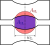
\includegraphics{lendl-2-roll}
        \caption{Lendl Areas for a Two-Roll Pass}
        \label{fig:lendl-2-roll}
    \end{figure}

    The original method by \textcite{Lendl_1948a, Lendl_1948b, Lendl_1949} was defined for two-roll passes of classic elongation passes.
    The basic idea is to define a contact width of incoming profile and rolls by intersection of their contours, as shown in \autoref{fig:lendl-2-roll}.
    This width is commonly referred to as Lendl's width $w_{\mathrm L}$.
    Accordingly, the two areas $A_{0\mathrm L}$ and $A_{1 \mathrm{L}}$ are called Lendl's areas, which are the respective profile cross-sections clipped symmetrically at $w_{\mathrm L}$.

    The heights of the equivalent flat pass are defined as

    \begin{equation}
        h'_{i} = \frac{A_{i \mathrm L}}{w_{\mathrm L}}
        \label{eq:equivalent_height2}
    \end{equation}

    For the equivalent width \textcite{Mauk_Kopp_1982} suggest to use the maximum width of the profile.
    This is implemented with this plugin.


    \subsection{Three-Roll Passes}

    \begin{figure}
        \centering
        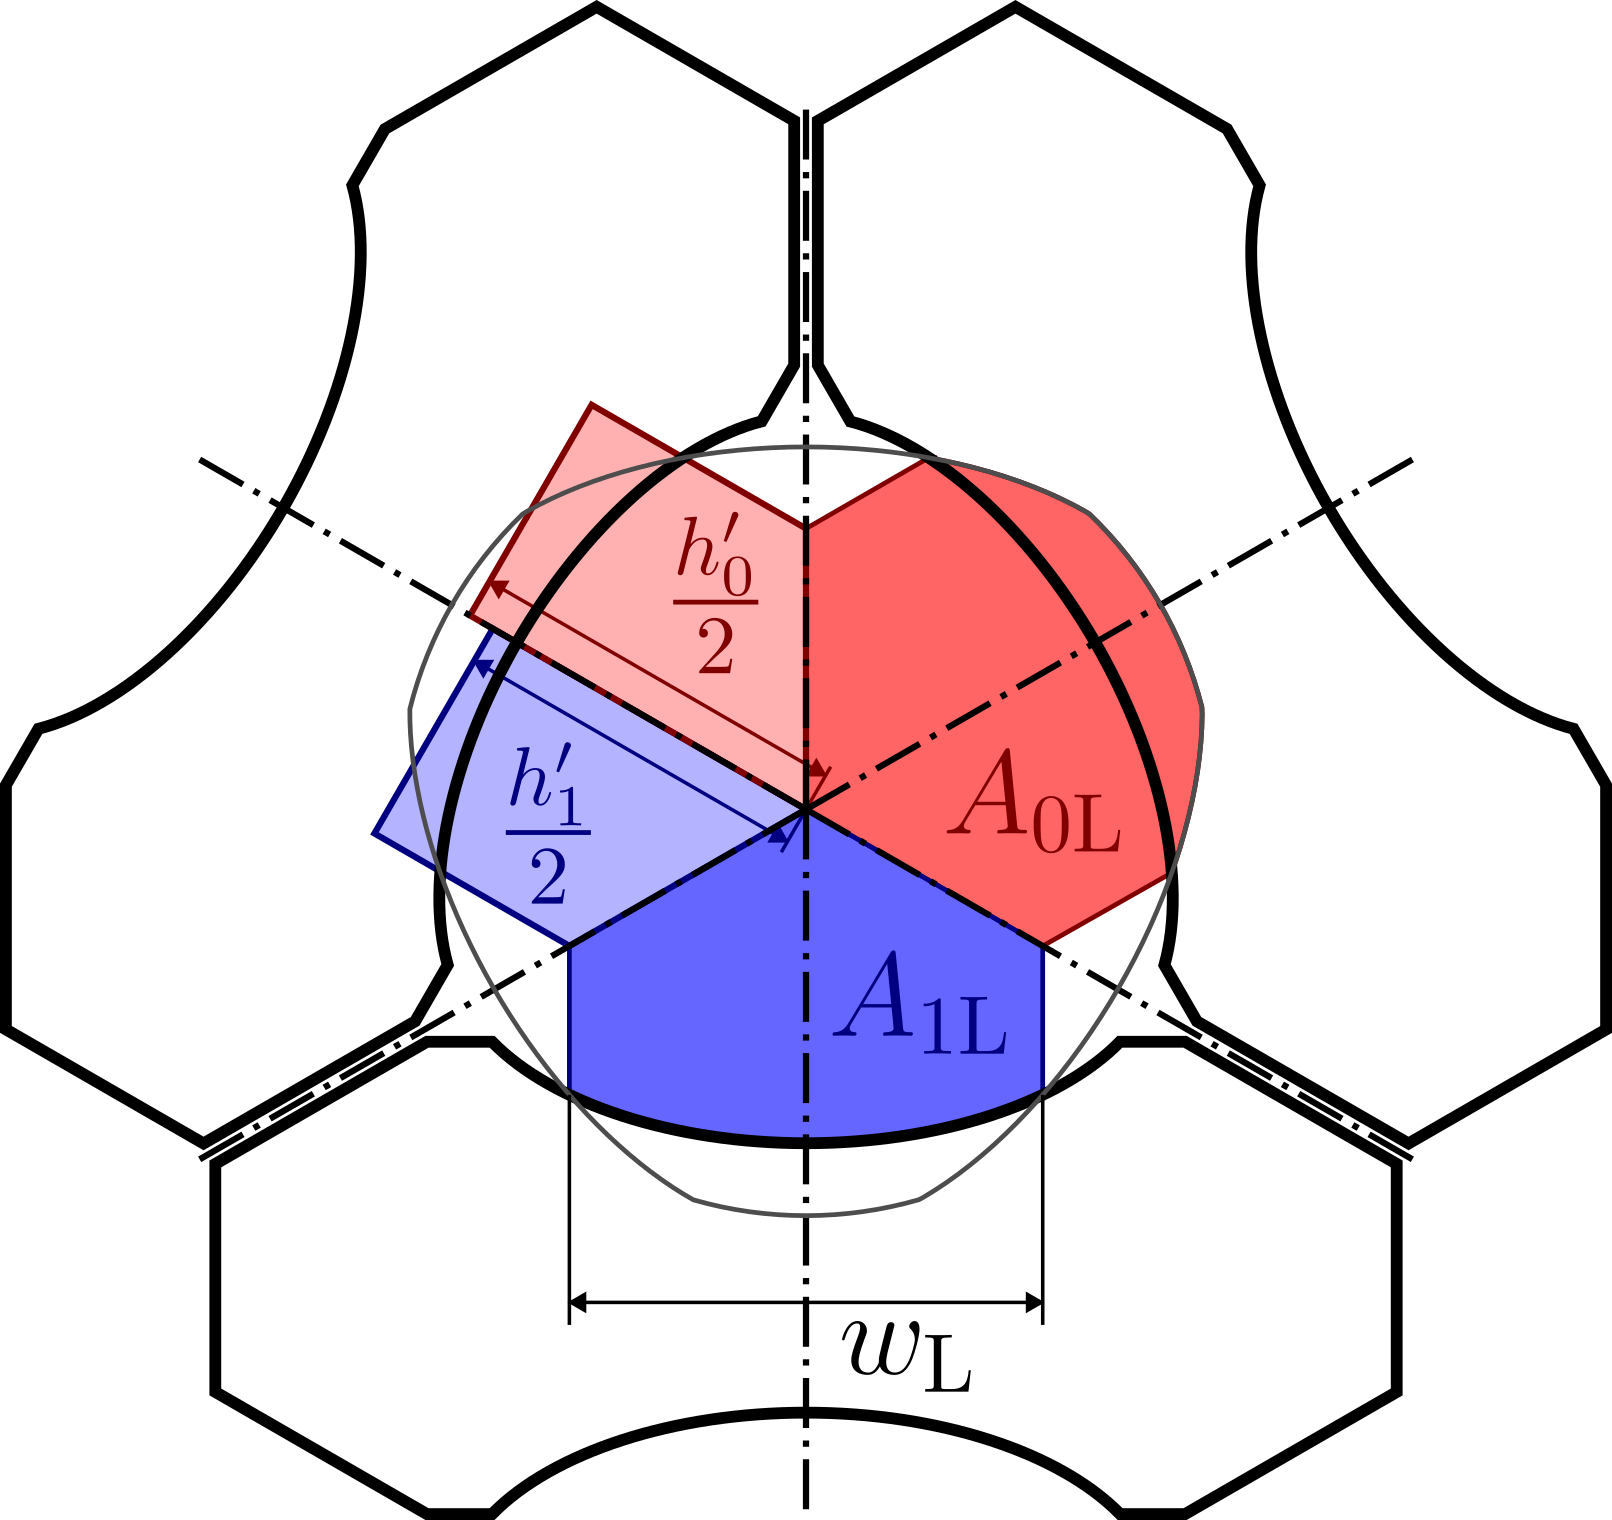
\includegraphics{lendl-3-roll}
        \caption{Lendl Areas, Widths and Heights According to~\cite{Overhagen2014}}
        \label{fig:lendl-3-roll}
    \end{figure}

    For roll passes working with a three-roll system, the approach is slightly different due to the 3-fold symmetry as shown in \autoref{fig:lendl-3-roll}.
    Lendl's method for 3-roll passes was proposed by \textcite{Overhagen2014}.
    The method shown there is implemented with this plugin, but note the difference to the definition of widths and heights in PyRolL\@.

    The equivalent heights are calculated using

    \begin{equation}
        h'_i = 2 \frac{A_{i\mathrm L} + \frac{\sqrt 3 w_{\mathrm L}^2}{12}}{w_{\mathrm L}}
        \label{eq:equivalent_height3}
    \end{equation}


    \section{Usage instructions}\label{sec:usage-instructions}

    The plugin can be loaded under the name \py/pyroll.lendl_equivalent_method/.
    The functionality of the plugin should work out of the box without provision of further data on units and incoming profile.

    The plugin provides hook functions for \py/RollPass.Profile.euqivalent_width/ and \py/RollPass.Profile.equivalent_height/ using the calculation method above.
    Two hooks are defined additionally: \py/RollPass.lendl_width/ representing Lendl's width $w_{\mathrm L}$ and \py/RollPass.Profile.lendl_section/ representing the geometry of Lendl's areas $A_{i \mathrm L}$.
    The latter return a \py/shapely.Polygon/ object to be able to access geometric data aside the area itself.
    Therefore, the name \texttt{section} was chosen to distinguish from the pure numeric area value.

    \printbibliography


\end{document}